\documentclass[12pt]{article}
\usepackage[T2A]{fontenc}
\usepackage[utf8]{inputenc}
\usepackage{multirow}
\usepackage{caption}
\usepackage{subcaption}
\usepackage{amsmath}
\usepackage{changepage}
\usepackage{graphicx}
\usepackage{float}
\usepackage[english,russian]{babel}
\usepackage{amsmath, amsfonts, amssymb, amsthm, mathtools}
\usepackage{xcolor}
\usepackage{array}
\usepackage{hyperref}
\usepackage[top = 1.5cm, left = 1.5 cm, right = 1.5 cm, bottom = 3 cm]{geometry}
\graphicspath{ {./images/} }
 
\title{Определение погонной плотности струны}
\author{Шахматов Андрей, Б02-304}
\date{\today}
  
\begin{document}
\begin{titlepage}
    \begin{center}
        {\large МОСКОВСКИЙ ФИЗИКО-ТЕХНИЧЕСКИЙ ИНСТИТУТ (НАЦИОНАЛЬНЫЙ ИССЛЕДОВАТЕЛЬСКИЙ УНИВЕРСИТЕТ)}
    \end{center}
    \begin{center}
        {\large Физтех-школа физики и исследований им. Ландау}
    \end{center}
    
    
    \vspace{3cm}
    {\huge
        \begin{center}
            \textbf{Определение погонной плотности струны колебательным методом}
        \end{center}
    }
    \vspace{2cm}
    \begin{flushright}
        {\LARGE Автор:\\ Шахматов Андрей Юрьевич \\
            \vspace{0.2cm}
            Б02-304}
    \end{flushright}
    \vspace{7 cm}
    \begin{center}
        Долгопрудный 2023
    \end{center}
\end{titlepage}

% \maketitle

\begin{abstract}
Исследованы резонансные частоты поперечных колебаний струны в зависимости от её силы натяжения. Найдены скорости распространения волны по струне
для различных длин натяжения струны. Рассчитана погонная плотность струны с погрешностью $1\%$. Проведён сравнительный анализ полученнного результата с табличной величиной,
в результатае которого рассчитанная величина погонной плотности совпала с табличной в пределах погрешности.
\end{abstract}

\tableofcontents

\section{Введение}
Изучение физических свойств струн является важным направлением современной науки. Струны широко применяются в различных областях, 
включая музыку и инженерию. Одним из ключевых параметров струны, который требует особого внимания, является ее погонная плотность.
Погонная плотность струны определяет ее массу на единицу длины. Классическим методом измерения погонной плотности является измерение массы
струны большой длины и нахождения погонной плотности как отношения полученной массы к длине струны. Однако В для очень лёгких или дорогих материалов
данный метод не является точным, из-за невозможности получить струну достаточной длины. Существуют иные методы измерения погонных плотностей струн,
и одним из таких является метод измерения погонной плотности струны при помощи исследований её поперечных колебаний. Цель настоящей работы заключалась
в определении погонной плотности струны при помощи исследований её поперечных колебаний.

\section{Методика}
\subsection{Поперечные колебания струны}
Рассмотрим собственные колебания струны длины $l$, закреплённой между двумя неподвижными опорами. При некоторых параметрах системы уравнение колебаний струны
будет представлять стоячую волну: $y(x, t) = Acos(kx)cos(wt + \phi)$. В таком случае между опорами должно помещаться целое число длин полуволн 
$\frac{\lambda}{2}$:
\begin{equation}\label{eq:1}
    n\frac{\lambda}{2} = l
\end{equation}
Тогда частоты собственных колебаний струны выражаются через скорость распространения поперечных волн $u$ и длину нити $l$:
\begin{equation}\label{eq:2}
    \nu_n = n\frac{u}{2l}
\end{equation}
Скорость распространения поперечных волн выражается через силу натяжения нити $F$ и погонную плотность $\rho_l$:
\begin{equation}\label{eq:3}
    u = \sqrt{\frac{F}{\rho_l}}
\end{equation}
Тогда ислледуя резонансные частоты для различных сил натяжения струны возможно найти скорость распространения поперечных волн для каждой
силы натяжения, из чего найти погонную плотность струны как коэффициент наклона графика $u^2(F)$.

В эксперименте использовалась установка, изображённая на рисунке \ref{fig:1}. Для поддержания колебаний использовался электромагнит, подключённый 
к генератору переменного напряжения. В случае высокой добротности системы коэффициент бегучести волны будет много меньше 1. Тогда можно считать, что
вынужденные колебания струны совпадают с её собственными колебаниями.
\begin{figure}
    \begin{center}
        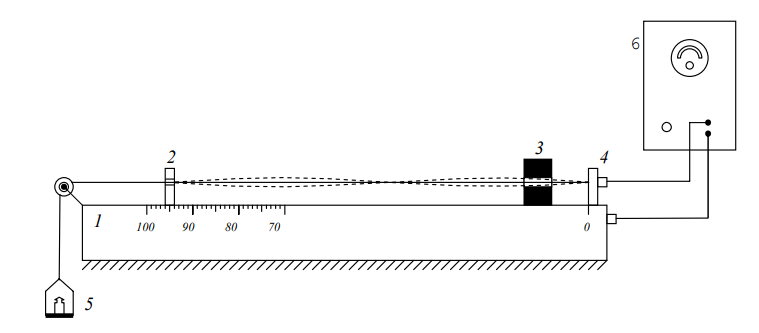
\includegraphics[width=0.7\textwidth]{img.png}
    \end{center}
    \caption{Схема экспериментальной установки. 1 - металлическая рейка, на которой закреплена струна,
        2 - зажим, регулирующий зажатие струны, 3 - магнит, поддерживающий колебания в струне, 4 - опора, на которой закрепляется струна,
        5 - подвес с грузами для изменения амплитуды колебаний, 6 - генератор переменного напряжения, подключённый к электромагниту.}
    \label{fig:1}
\end{figure}

\section{Результаты и их анализ}
Резонансные частоты находились при помощи осцилографа, подключённого в двухканальном режиме к генератору и струне. При таком подключении в 
случае резонанса на экране осцилографа должен быть неподвижный эллипс, такой рисунок означает установление резонанса. Все измерения проводились 
при амплитуде колебаний $300$ мВ. Для нечётных колебаний измерение проводились в центре струны. Для чётных колебаний измерение проводилось на 
расстоянии $\frac{l}{2n}$ от центра струны. Данные результатов измерений представлены в таблице \ref{tab:1}.
Построены графики зависимости резонансных частот в зависимости от числа полуволн $n$ (Рис. \ref{fig:2})
\begin{figure}[H]
    \begin{center}
        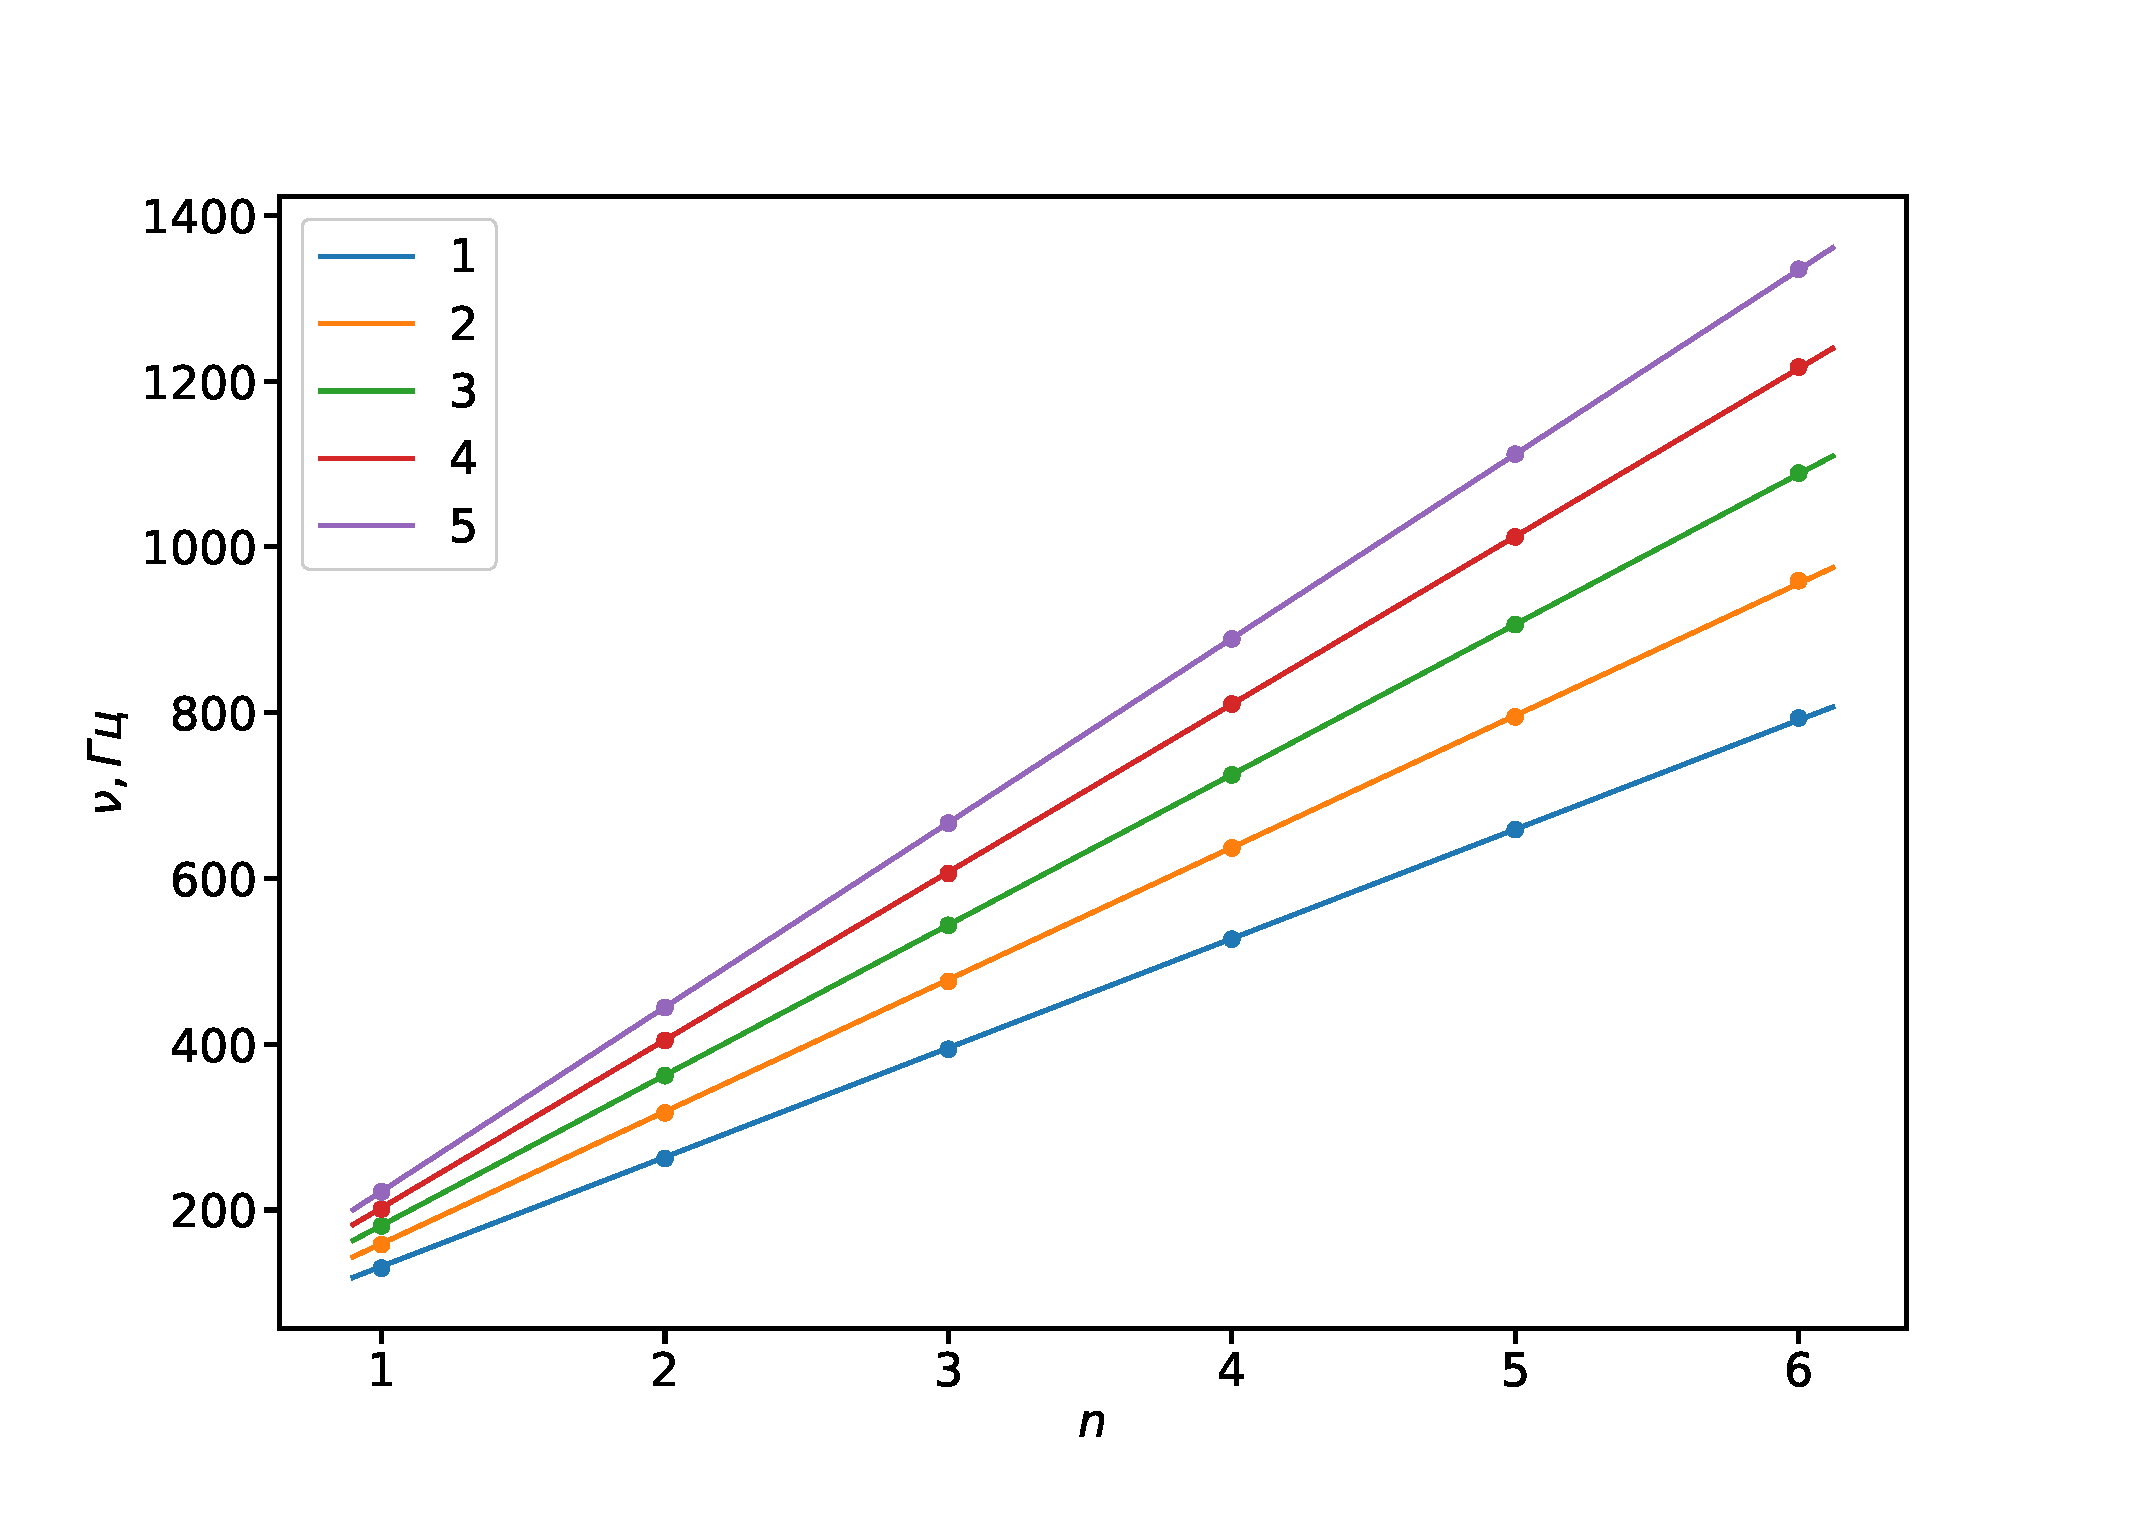
\includegraphics[width=0.9\textwidth]{gr0.eps}
    \end{center}
    \caption{Графики зависимостей резонансных частот при различных натяжениях нити. Номерами обозначены прямые, соответствующие номерам натяжениям
        из таблицы \ref{tab:1}.}
    \label{fig:2}
\end{figure}
Из каждой зависимости $\nu(n)$ для каждого $F$ из коэффициента наклона графика найдём скорость распространения поперечных волн $u = k_n\cdot2l$, 
где $k_n$ - коэффициент наклона соответствующего графика. Полученые значения скоростей представлены в таблице \ref{tab:2}.
Построен график зависимости $u^2(F)$(Рис. \ref{fig:3}) 
\begin{figure}[H]
    \begin{center}
        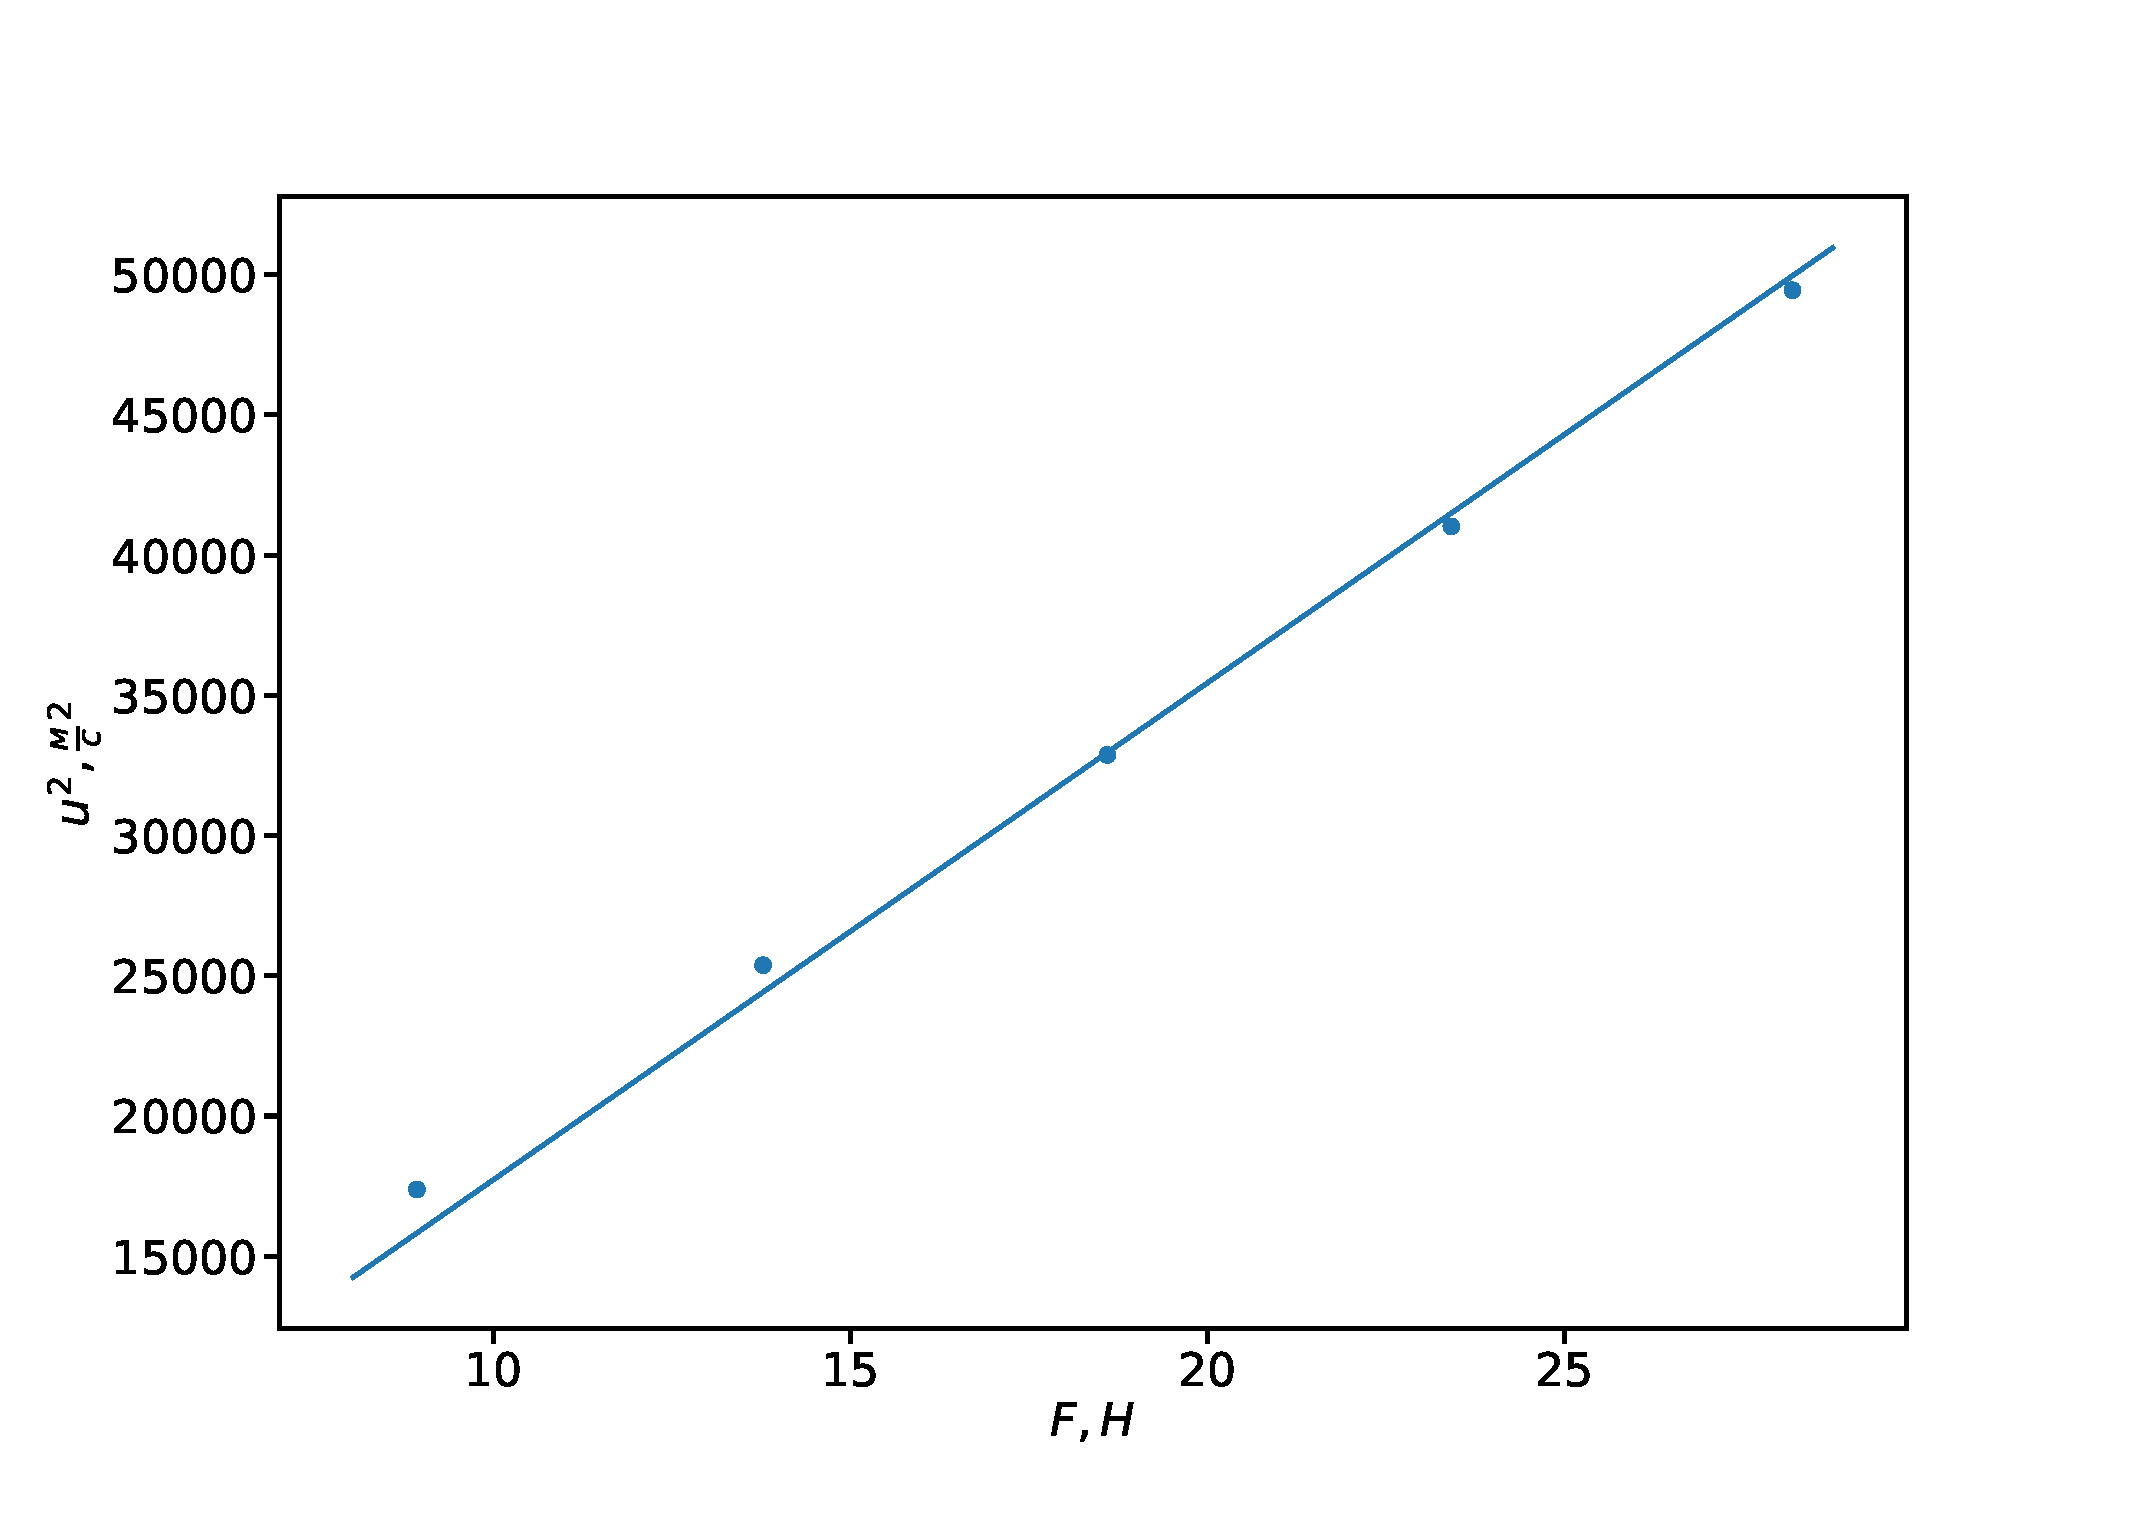
\includegraphics[width=0.9\textwidth]{gr.eps}
    \end{center}
    \caption{График зависимости квадрата скорости распространения поперечных волн $u^2$ от силы натяжения струны $F$. Кресты погрешностей
        по оси $u^2$ много меньше масштаба графика, потому не были нанесены. Кресты погрешностей по оси $F$ много меньше максштаба графика, 
        потому не были нанесены.}
    \label{fig:3}
\end{figure}
Зависимости $\nu(n)$ (Рис. \ref{fig:2}) и зависимость $u^2(F)$ (Рис. \ref{fig:3}) оказалась линейной, потому использованная модель колебаний 
струны является корректной. Из коэффициента наклона графика \ref{fig:3} $k$ найдена погонная плотность струны 
$\rho_l = \frac{1}{k} = (5.64 \pm 0.07) \cdot 10^{-4} \frac{\textrm{кг}}{\textrm{м}}$. Полученная погонная плотность струны совпала с табличной
$\rho_{lt} = 5.68 \cdot 10^{-4} \frac{\textrm{кг}}{\textrm{м}}$ в пределах погрешности. Причём относительная погрешность результата составила $1\%$.

\section{Выводы}
Полученная погонная плотность струны совпала с табличным занчением, причём при использовании предложенного метода можно достичь точности измерения
$1\%$.

\section{Использованная литература}
\begin{thebibliography}{9}
    \bibitem{LabBook}
    Лабораторный практикум по общей физике, Том 1, под редакцией А. Д. Гладуна
\end{thebibliography}

\section{Приложения}
\subsection{Измерения резонансных частот при различных натяжениях струны} \label{app_1}
\begin{table}[H]
    \centering
    \begin{tabular}{|l|r|r|r|r|r|r|r|r|r|r|}
        \hline
        Номер измерения & $F, H$ & $\nu_1, \textrm{ Гц}$ & $\nu_2, \textrm{ Гц}$ & $\nu_3, \textrm{ Гц}$ & $\nu_4, \textrm{ Гц}$ & $\nu_5, \textrm{ Гц}$ & $\nu_6, \textrm{ Гц}$ \\
        \hline
        1               & 8.93   & 129.75                & 261.9                 & 393.85                & 526.69                & 658.82                & 793.54                \\
        2               & 13.78  & 158.2                 & 317.1                 & 475.7                 & 636.7                 & 794.92                & 959.2                 \\
        3               & 18.60  & 180.7                 & 362.0                 & 543.4                 & 724.82                & 906.2                 & 1089.0                \\
        4               & 23.42  & 201.1                 & 404.3                 & 605.83                & 810.32                & 1012.1                & 1217.0                \\
        5               & 28.19  & 221.8                 & 444.1                 & 666.7                 & 888.89                & 1111.9                & 1335.0                \\
        \hline
        
    \end{tabular}
    \caption{Измерения резонансных частот $\nu_n$ при различных натяжениях струны $F$}
    \label{tab:1}
\end{table}

\subsection{Измерения скорости распространения поперечных волн в струне от силы натяжения} \label{app_2}
\begin{table}[H]
    \centering
    \begin{tabular}{|l|r|r|r|r|r|r|r|r|r|r|}
        \hline
        $u, \frac{\textrm{м}}{\textrm{с}}$ & $u^2, \frac{\textrm{м}^2}{\textrm{с}^2}$ & $F, H$ \\
        \hline
        131.84                             & 17381.09                                 & 8.93   \\
        159.30                             & 25375.78                                 & 13.78  \\
        181.31                             & 32873.19                                 & 18.60  \\
        202.53                             & 41021.69                                 & 23.42  \\
        222.36                             & 49445.92                                 & 28.19  \\
        \hline
        
    \end{tabular}
    \caption{Измерения скорости распространения поперечных волн в струне $u$ от силы натяжения $F$}
    \label{tab:2}
\end{table}
\subsection{Расчёт коэффициентов наклона и их погрешностей}\label{app_3}
Формула для расчёта коэффициента и погрешности:
$$k = \frac{\overline{x}\overline{y}}{\overline{x^2}}$$
$$\sigma_k = \frac{1}{\sqrt{n}}\sqrt{\frac{\overline{y^2}}{\overline{x^2}} - k^2}$$
В этой формуле считается, что известно, что y(0) = 0
\end{document}